\vspace*{1em}

{\bf Pythagorean Triples.}
\begin{definition}
Let $a,b,c$ be positive integers. Say $(a,b,c)$ is a Pythagorean triple if $a^2 + b^2 = c^2$.
\[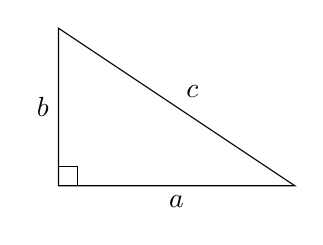
\begin{tikzpicture}
        \draw[]  (0, 0) coordinate (A) 
        -- node[left] {$b$} (0,2) coordinate (C) 
        -- node[above right] {$c$} (3,0) coordinate (B) 
        -- node[below] {$a$}  (-0.007,0);
       \draw (0,7pt) -- ++(7pt,0) -- ++(0,-7pt);
      \end{tikzpicture}\]
\emph{e.g.}\quad $(3,4,5),\ (5,12,13)$
\end{definition}

\vspace*{1.5em}

{\bf Goal.} Find \emph{all} Pythagorean triples.

\vspace*{2em}

{\bf Geometric Strategy.} Start with equation
\[a^2 + b^2  = c^2\]
Dividing both sides by $c^2$, and letting $x \coloneqq a/c$ and $y \coloneqq b/c$. Then
\[x^2 + y^2 = 1\]
Since $a,b,c$ are positive integers, $x,y$ are rational and $(x,y)$ lies on the unit circle! In other words, any Pythagorean triple gives rise to a rational point (points with rational coordinates) on the unit circle.\\
\\
For such a point $(x,y)$, consider the line passing through $(x,y)$ and $(-1,0)$. What can you say about the slope of this line?
\[\begin{tikzpicture}[scale=2]
    \draw[<->,thick] (-1.7,0)--(1.7,0);
    \draw[<->,thick] (0,-1.5)--(0,1.5);
    \draw[thick](0,0) circle (1);
	\draw[<->,thick,>=stealth, color=firebrick] (-1.4,-0.2)--(1.5,1.25);   
	\draw[<->,thick,>=stealth, color=indigo] (-1.5,-0.1)--(2,0.6);   
    \fill (-1,0) circle (1pt);
    \fill (0.6,0.8) circle (1pt);
    \fill (0.923076923,0.384615385) circle (1pt);
    \node[] at (-1.3,0.2) {\footnotesize$(-1,0)$};
    \node[] at (0.6,1.05) {\footnotesize$(x,y)$};
    \node[] at (1.7,0.7) {\color{indigo} \small $L_t$};
\end{tikzpicture}\]
Suppose we draw a line $L_t$ through $(-1,0)$ with rational slop $t$, what we can say about the point at which it intersects the unit circle $C$?

\vspace*{1em}

\begin{proposition}
There's a bijection, where $P_0 = (-1,0)$
\[\begin{tikzcd}
\set{P = (x,y) \in \qq^2\ \Bigg\vert \begin{minipage}{0.13\textwidth}
\begin{center}
$P \neq P_0$\\[0.2em] $x^2 + y^2 = 1$
\end{center}
\end{minipage}}
 \arrow[r,shift left=2,"{\color{firebrick}f}"] &[1em]  \arrow[l,shift left=2,"{\color{indigo}g}"] \set{\begin{minipage}{0.2\textwidth}
\begin{center}
lines through $P_0$ with rational slope $t$.
\end{center}
\end{minipage}}
\end{tikzcd}\]
\end{proposition}
\begin{proof}
Define
\[{\color{firebrick}f}:P \mapsto \text{the line $L$ passing through $P_0$ and $P = (x,y)$}\]
Note that $L$ has rational slope: $\dfrac{y - 0}{x - (-1)} = \dfrac{y}{x+1}$ is rational since $x,y$ are rational numbers.\\
\\
We now describe ${\color{indigo}g}$: let $L_t$ be the line through $P_0$ with rational slop $t$. Then $L_t$ is defined by the equation \[y = t(x-(-1)) = t(x+1).\]
Let $(u,v) \in L_t \cap C$ then $v = t(u+1)$ and
\begin{align*}
u^2 + (t(u+1))^2 &= 1\\[0.5em]
u^2 + t^2(u^2 + 2u + 1) &= 1\\[0.5em]
(1+t^2)u^2 + 2ut^2 + (t^2 - 1) &= 0\\[0.5em]
u^2 + \left(\frac{2t^2}{1+t^2}\right)u + \left(\frac{t^2-1}{1+t^2}\right) &= 0
\end{align*}
As a quadratic equation in $u$, the equation above necessarily has two roots, say $\alpha$ and $\beta$. Crucial point is that $\alpha = -1$ is a root since $(-1,0) \in L_t\cap C$. Since we know that
\[\alpha\beta = \frac{t^2-1}{1+t^2},\quad \text{therefore }\ \beta = \frac{1-t^2}{1+t^2}\]
is the other root, i.e. $u = \dfrac{1-t^2}{1+t^2}$ is the $x$-coordinate of the other point in $L_t \cap C$. Then
\begin{align*}
v = t(u+1) &= t\left(\frac{1-t^2}{1+t^2} + 1\right)\\[0.5em]
&= \frac{2t}{1+t^2}
\end{align*}
Define ${\color{indigo}g}(L_t) = \left(\dfrac{1-t^2}{1+t^2},\dfrac{2t}{1+t^2}\right) \in \qq^2$.\\
\\[0.5em]
One readily checks $f$ and $g$ are inverses of each other.
\end{proof}

\emph{e.g.}\quad $t = 1/5$ corresponds to the Pythagorean triple $(12,5,13)$.
\begin{align*}
g(L_{1/5}) &= \left(\frac{1-(1/5)^2}{1+(1/5)^2},\frac{2(1/5)}{1+(1/5)^2}\right)\\[0.5em]
&= \left(\frac{24}{26},\frac{10}{26}\right) = \left(\frac{12}{13},\frac{5}{13}\right)
\end{align*}

%\vspace*{2.5em}

\begin{center}
{\Large Modular Arithmetic}
\end{center}

Sometimes, the remainder left after division can tell us a lot!
\begin{proof}[e.g.]\renewcommand{\qedsymbol}{}
\begin{itemize}
\item[(1)] Is $317 \times 694 = 219996$? \emph{No, since the last digit should be $8$. $317 \times 694 = 219998$.}
\end{itemize}
\begin{itemize}[leftmargin=4.4em]
\item[(2)] Is $9217$ a square of an integer? Equivalently, does $x^2 = 9217$ have an integer solution? \emph{No, because the last digit of a square can only be $0,1,4,5,6$ or $9$.}
\item[(3)] Does the equation 
\begin{align*}\label{intsol}
x^2 + y^2 &= 1234567 \tag{$\dagger$}
\end{align*}
have an integer solution?
\end{itemize}
\end{proof}

\begin{definition}
Let $m$ be a positive integer (called a \emph{modulus}). Say that two integers $a$ and $b$ are \emph{congruent modulo $m$}, written as
\[a\equiv b\modar{m},\]
if $m\mid (a-b)$, or equivalently $m\mid (b-a)$.\\
\\
Congruence modulo $m$ is an equivalence relation.
\end{definition}
\emph{e.g.} $317 \equiv 17\modar{10} \equiv 7\modar{10} \equiv -3\modar{10}$

\vspace*{1.5em}

\begin{proposition}\label{modps}
Let $m$ be a modulus, and $a,b,c,d$ are integers such that
\[a\equiv b\modar{m} \quad \text{and} \quad c\equiv d\modar{m}.\]
Then $a+c \equiv b+d\modar{m}$ and $ac \equiv bd\modar{m}$.
\end{proposition}
\begin{proof}
(product) By assumption, 
\begin{align*}
a-b &= mr,\quad \text{for some $r\in \zz$}; & c-d &= ms,\quad \text{for some $s\in \zz$}
\end{align*}
Then 
\begin{align*}
ac &= (b+mr)(d+ms)\\[0.5em]
&= bd + m^2rs + m(dr + bs)\\[0.5em]
ac - bd &= m(mrs + dr + bs)
\end{align*}
Therefore $m\mid (ac-bd)$, and hence $ac\equiv bd \modar{m}$.
\end{proof}

\vspace*{1em}

\begin{definition}
Let $x$ be an integer and $m$ a modulus, the \emph{natural representative of $x$ modulo $m$} is the remainder $r$ left under the division algorithm
\[x = qm + r,\quad 0 \leq r < m.\]
Therefore $x \equiv r\modar{m}$.
\end{definition}
\begin{proof}[e.g.]\renewcommand{\qedsymbol}{}
\begin{itemize}
\item[(1)] Compute the natural representative modulo $10$ of $1234567 \cdot 314159265$.\\[0.5em]
\hspace*{1.9em}\emph{Hard way:} Multiply this number and find out.\\[0.5em]
\hspace*{1.9em}\emph{Easy way:} Using Proposition \ref{modps},
\begin{align*}
1234567 \cdot 314159265 &\equiv 7\cdot 5\modar{10}\\[0.5em]
&\equiv 35\modar{10}\\[0.5em]
&\equiv 5\modar{10}
\end{align*}
\end{itemize}
\begin{itemize}[leftmargin=4.4em]
\item[(2)] Compute the natural representative modulo $13$ of $24^5$.\\[0.5em]
First, $24 = 13 + 11 \equiv 11\modar{13} \equiv -2\modar{13}$. Now, by Proposition \ref{modps},
\begin{align*}
28^5 \equiv (-2)^5\modar{13} &\equiv -32\modar{13}\\[0.5em]
&\equiv 39 - 32\modar{13}\\[0.5em]
&\equiv 7\modar{13}
\end{align*}
\item[(3)] Compute the natural representative modulo $7$ of $2^{10}$.\\
\\
(Attempt) $10 = 7 + 3\modar{7}$, and so
\[2^{10} \equiv 2^3\modar{7} \equiv 8\modar{7} \equiv 1\modar{7}\]
Incorrect! $2^{10} \not\equiv 2^3\modar{7}$.\\
\\
(Actual) $2\equiv 2\modar{7},\ 2^2\equiv 4\modar{7},\ 2^3\equiv 8\modar{7}\equiv 1\modar{7}$. So, 
\[2^{10} = 2^3\cdot 2^3\cdot 2^3\cdot 2\equiv 1\cdot 1\cdot 1\cdot 2 2\modar{7}\equiv 2\modar{7}\]
\emph{Caution.} In general, $b \equiv c\modar{m}$ does \emph{not} imply $a^b\equiv a^c\modar{m}$.
\end{itemize}
\end{proof}

%\vspace*{1em}

\begin{proposition}
Let $N$ be a positive integer, and $S$ be the sum of its digits. Then $N \equiv S\modar{9}$, and hence also $N \equiv S\modar{3}$.
\end{proposition}
\begin{proof}
Let $N = d_0 + d_1\cdot 10 + \cdots + d_k\cdot 10^k$, e.g. $247 = 7 + 4\cdot 10 + 7\cdot 100$. Then
\begin{align*}
N &= d_0 + d_1\cdot 10 + \cdots + d_k\cdot 10^k\\[0.5em]
&\equiv d_0 + d_1\cdot 1 + \cdots + d_k\cdot 1^k\modar{9},\quad\text{by Proposition \ref{modps}}\\[0.5em]
&\equiv d_0 + d_1 + \cdots + d_k\modar{9}\\[0.5em]
&\equiv S\modar{9}\\[-3em]
\end{align*}
\end{proof}
\emph{e.g.}\quad Note $247 \equiv 2 + 4 + 7 \modar{9} \equiv 13\modar{9} \equiv 1 + 3\modar{9} \equiv 4\modar{9}$.

\vspace*{3em}

Back to example \refp{intsol}. Does the equation $x^2 + y^2 = 1234567$ have an integer solution?
\begin{proof}[Answer]
Strategy is to look at the equation modulo $4$.
\begin{itemize}[leftmargin=*]
\item[] If $z$ is an even integer, then $z = 2n$ for some integer $n$, and so 
\[z^2 = (2n)^2 = 4n^2 \equiv 0\modar{4}\]
\item[] If $z$ is an odd integer, then $z = 2m+1$ for some integer $m$, and so 
\[z^2 = (2m+1)^2 = 4m^2 + 4m + 1 \equiv 1\modar{4}\]
\end{itemize}
Therefore, if a solution $(x,y)$ existed then $x,y \equiv 0,1\modar{4}$ and so $x^2 + y^2 \equiv 0,1,2\modar{4}$.\\
\\
But 
\begin{align*}
1234567 &= 12345\cdot 100 + 67\\[0.5em]
&\equiv 67\modar{4}\\[0.5em]
&\equiv 64 + 3\modar{4}\\[0.5em]
&\equiv 3\modar{4}
\end{align*}
Thus, no solution exists.
\end{proof}

\vspace*{2em}

{\bf Solving Quadratic Equations, so far.}
\begin{itemize}[itemsep = 2em]\label{quadeqex}
\item[(1)] $x^2 + y^2 = 1234567$ has no integer solutions.
\item[(2)] $x^2 + y^2 = z^2$ has infinitely many integer solutions, since we found all the rational solutions to the equation $X^2 + Y^2 = 1$.
\[\begin{tikzpicture}[scale=2]
    \draw[<-,thick] (-1.7,0)--(-1,0);
    \draw[<->,thick] (0,-1.5)--(0,1.5);
    \draw[thick](0,0) circle (1);
    \fill (-1,0) circle (1pt);
	\draw[->,thick,>=stealth, color=teal] (-1,0)--(-0.3,1.4); %t = 2
    \fill[color=firebrick] (-0.6,0.8) circle (1pt); %t = 2
    \draw[->,thick,>=stealth, color=teal] (-1,0)--(0.3,1.3); %t = 1
    \fill[color=firebrick] (0,1) circle (1pt); %t = 1
    \draw[->,thick,>=stealth, color=teal] (-1,0)--(0.9,0.95); %t = 1/2
    \fill[color=firebrick] (0.6,0.8) circle (1pt); %t = 1/2
    \draw[->,thick,>=stealth, color=teal] (-1,0)--(1.2,0.55); %t = 1/4
    \fill[color=firebrick] (0.882352941,0.470588235) circle (1pt); %t = 1/4
    \draw[->,thick,>=stealth, color=teal] (-1,0)--(1.7,0); %t = 0
    \fill[color=firebrick] (1,0) circle (1pt); %t = 0
	\draw[->,thick,>=stealth, color=teal] (-1,0)--(-0.3,-1.4); %t = -2
    \fill[color=firebrick] (-0.6,-0.8) circle (1pt); %t = -2
    \draw[->,thick,>=stealth, color=teal] (-1,0)--(0.3,-1.3); %t = -1
    \fill[color=firebrick] (0,-1) circle (1pt); %t = -1
    \draw[->,thick,>=stealth, color=teal] (-1,0)--(0.9,-0.95); %t = -1/2
    \fill[color=firebrick] (0.6,-0.8) circle (1pt); %t = -1/2
    \draw[->,thick,>=stealth, color=teal] (-1,0)--(1.2,-0.55); %t = -1/4
    \fill[color=firebrick] (0.882352941,-0.470588235) circle (1pt); %t = -1/4
    \fill (-1,0) circle (1pt);
	\node[] at (-1.3,0.15) {\footnotesize$(-1,0)$};
    \node[] at (-0.4,1.5) {\footnotesize $t=2$};
    \node[] at (-0.475,-1.5) {\footnotesize $t=-2$};
    \node[] at (0.525,1.35) {\footnotesize $t=1$};
    \node[] at (0.6,-1.35) {\footnotesize $t=-1$};
    \node[] at (1.2,0.95) {\footnotesize $t=1/2$};
    \node[] at (1.275,-0.95) {\footnotesize $t=-1/2$};
    \node[] at (1.5,0.55) {\footnotesize $t=1/4$};
    \node[] at (1.575,-0.55) {\footnotesize $t=-1/4$};
    \node[] at (1.95,0) {\footnotesize $t=0$};
	\draw[->,>=stealth,thick,color=indigo] (1.5,1) (2.5,1) arc(225:135:-1.5);
    \node[] at (3.5,0) {\footnotesize\begin{tabular}{c}\emph{method of}\\ \emph{sweeping lines}\end{tabular}};
\end{tikzpicture}\]
\item[(3)] Find all rational solutions to $x^2 + y^2 = 3$.
\begin{itemize}
\item[(i)] No obvious ``pivot" with rational coordinates.
\[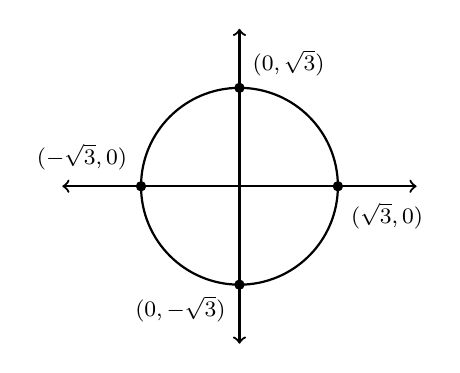
\begin{tikzpicture}[scale=1.25]
    \draw[<->,thick] (1.8,0)--(-1.8,0);
    \draw[<->,thick] (0,-1.6)--(0,1.6);
    \draw[thick](0,0) circle (1);
    \fill (-1,0) circle (1.5pt);
    \fill (1,0) circle (1.5pt);
    \fill (0,-1) circle (1.5pt);
    \fill (0,1) circle (1.5pt);
	\node[] at (-1.6,0.3) {\footnotesize$(-\sqrt{3},0)$};
	\node[] at (1.5,-0.3) {\footnotesize$(\sqrt{3},0)$};
	\node[] at (0.5,1.25) {\footnotesize$(0,\sqrt{3})$};
	\node[] at (-0.6,-1.25) {\footnotesize$(0,-\sqrt{3})$};
\end{tikzpicture}\]
\item[(ii)] Look at integer solutions.\\[0.5em]
Since $x^2,y^2 \geq 0$ and $x^2 + y^2 = 3$, necessarily $0 \leq x^2,y^2 \leq 3$. So, if $x,y \in \zz$, then $x,y = 0,\pm 1$. But none of these solve $x^2 + y^2 = 3$, and therefore there are no integer solutions\\[0.5em]
Alternatively, you can reduce mod $4$ and proceed as in (1).\\
\item[(iii)] How about rational solutions?\\[0.5em]
Assume towards a contradiction that $(u,v) \in \qq^2$ is a solution of $x^2 + y^2 = 3$, i.e.
\begin{align*}\label{eq81}
u^2 + v^2 = 3 \tag{$\star$}
\end{align*}
Let $c$ be the $\lcm$ of the denominators of $x$ and $y$ in their reduced form, and write
\begin{align*}\label{eq82}
u = \frac{a}{c},\quad v = \frac{b}{c} \tag{$\star\star$}
\end{align*}
{\small (\emph{e.g.} if $u = 3/10$ and $v = 4/15$, then $c = \lcm(10,15) = 30$; rewrite as $u = 9/30$ and $v = 8/30$.)}\\[0.5em]
Then $\gcd(a,b,c) = 1$ (see Problem \ref{Problem 8.1}) and $c\geq 1$.\\
\\
Rewriting \refp{eq81} using \refp{eq82}, we get
\begin{align*}\label{eq83}
\frac{a^2}{b^2} + \frac{b^2}{c^2} = 3 \iff a^2 + b^2 = 3c^2 \tag{$\star\star\star$}
\end{align*}
We want to now employ modular arithmetic, so for that a good modulus to choose will be $3$. Since $a,b,c \in \zz$, we get
\[a^2 + b^2 = 3c^2 \equiv 0 \modar{3}\]
Now, note that since $a \equiv 0,1,2\modar{3}$, therefore $a^2 \equiv 0,1\modar{3}$; similarly for $b^2\modar{3}$. Hence, the only way we have $a^2 + b^2 \equiv 0\modar{3}$ is if $a^2 \equiv b^2 \equiv 0\modar{3}$. Thus, $3\mid a^2$ and $3\mid b^2$, and so necessarily $3\mid a$ and $3\mid b$.\\
\\
Let $a = 3a_0$ and $b = 3b_0$, substituting this in \refp{eq83} gives us
\begin{align*}
3c^2 &= (3a_0)^2 + (3b_0)^2\\[0.5em]
c^2 &= 3(a_0^2 + b_0^2),\ \text{necessarily}
\end{align*}
Therefore $3\mid c^2$, and so necessarily $3\mid c$.\\
\\
Altogether we have $3\mid a,\,3\mid b$ and $3\mid c$; but we had $\gcd(a,b,c) = 1$. Hence we have arrived at a contradiction and thus $x^2 + y^2 = 3$ has no rational solutions.
\end{itemize}
\end{itemize}

\vspace*{0.5in}

\subsection{Problems}
\vspace{0.1in}

\begin{problem}\label{Problem 8.1}
Consider a pair of reduced fractions, $N_u/D_u$ and $N_v/D_v$ distinct as rational numbers. Let $c\coloneqq \lcm(D_u,D_v)$ and then suppose $c = D_um_u = D_vm_v$ for some integers $m_u,m_v$. Define $a = N_um_u$ and $b = n_vm_v$; prove that $\gcd(a,b,c) = 1$.
\end{problem}

\vspace{0.1in}

\begin{problem}\label{Problem 8.2}
Prove that there are infinitely many positive integer triples $(x,y,z)$ such that \[x^2 + 2y^2 = 3z^2.\]
{\footnotesize Hint: find an appropriate rational point that will act as a ``pivot", much like in the case of classifying Pythagorean triples that we saw in this lecture.}
\end{problem}

\vspace{0.1in}

\begin{problem}\label{Problem 8.3}
Let $N$ be a positive integer, and $A$ be the alternating sum of its digits. That is, if $N$ has a decimal expansion with units digit $u$, tens digit $t$, hundreds digit $h$ in units place, thousands digit $s$, then $A = u - t + h - s + \cdots$. Then $N \equiv S\modar{11}$.
\end{problem}

\vspace{0.1in}

\begin{problem}\label{Problem 8.4}\hfill
\begin{itemize}
\item[(a)] Let $n$ be any integer. Prove that $n^2$ is congruent to $0,\, 1$ or $4$ modulo $8$.
\item[(b)] Prove that there exists no integer solution $(x, y, z)$ to the equation
\[x^2 + y^2 + z^2 = 314159265358979323846264338327.\]
\item[(c)] Demonstrate that there are infinitely many positive integers that \emph{cannot} be written as a sum of three squares.
\end{itemize}
\end{problem}

\vspace{0.1in}

\begin{problem}\label{Problem 8.5}
Let $p$ be any prime number and let $a$ and $b$ be any two integers.
\begin{itemize}
\item[(a)] Prove that if $a \equiv b \modar{p}$, then $a^p \equiv b^p \modar{p^2}$.
\item[(b)] Prove that if $a \equiv b \modar{p}$, then $a^{p^2} \equiv b^{p^2} \modar{p^3}$.
\item[(b)] (challenge) Can you generalise?
\end{itemize}
\end{problem}

\vspace{0.1in}

\begin{problem}\label{Problem 8.6}
Compute (the natural representative of) $3^{10^{10^{10}}}\modar{7}$.
\end{problem}

\vspace{0.1in}

\begin{problem}\label{Problem 8.7}
Prove that a modulus $m$ is even if and only if there exists an integer $x$ such that $x \not\equiv 0\modar{m}$ and $x + x\equiv 0\modar{m}$.
\end{problem}

\vspace{0.1in}

\begin{problem}\label{Problem 8.8}
Recall the Fibonacci numbers from Problem \ref{Problem 6.2}. Prove that for all $n\geq 1$,
\[F_n \equiv 4^{n-1}(2^n - 1)\modar{11}\]
\end{problem}